\documentclass[10pt,twocolumn]{article}

\usepackage[UKenglish]{babel}
\usepackage{fontspec}
\usepackage{csquotes}
 \setmainfont{Times New Roman}
 
%\usepackage{times}
\usepackage{graphicx}
\usepackage{url}
\usepackage[a4paper, total={18cm, 24cm}]{geometry}
\usepackage[
backend=biber,
sortlocale=auto,
style=numeric,
citestyle=numeric,
maxnames=4
]{biblatex}
\usepackage[colorinlistoftodos,prependcaption,textsize=footnotesize]{todonotes}
\presetkeys%
    {todonotes}%
    {inline,backgroundcolor=yellow}{}

\addbibresource{iot-living-lab-refs.bib}

\setlength{\parindent}{0pt}
\setlength{\parskip}{6pt}

% correct bad hyphenation here
\hyphenation{op-tical net-works semi-conduc-tor}

\newcommand{\term}[1]{\textit{#1}}

\begin{document}

\title{I am not a number:\\
Towards participatory IoT monitoring in the workplace}



\author{\textbf{\textit{Cat Magill$^*$, Ewan Klein$^*$ and Simon Chapple$^\dagger$}}}
\date{}

\maketitle

% \begin{multicols}{1}
%   \begin{center}
%   $^*$School of Informatics, University of Edinburgh, \texttt{\{c.magill$\mid$ewan.klein\}@ed.ac.uk}
% $^\daggger$Information Services Group, University of Edinburgh, \texttt{Simon.Chapple@ed.ac.uk}
% \end{center}
% \end{multicols}

\todo{Fix affiliations}
\begin{abstract}
A dominant narrative around the Internet of Things (IoT) asserts that
value will be realized by using resources more efficiently and by
creating a better ‘user experience’.  We suggest that IoT initiatives,
particularly those involving monitoring, can create more value for
`users' and reduce the risk of adverse reactions to `overmonitoring'
if users are more actively involved in the design and communication
process.  On the basis of a small qualitative study of reactions by
employees to having their workplace monitored by networked sensors, we
offer three guidelines to help ensure that such initiatives
incorporate a broader set of values and beneficiaries. 
\end{abstract}



\section{Introduction}
\label{sec:introduction}

Early narratives of the Internet of Things (IoT) envisioned a ‘smart
planet’ where interconnected things communicate with each other
through a global information infrastructure, leading to efficient and
seamless operations and generating virtually unlimited opportunities
to develop new products and services based on insights from the data
collected and analysed \cite{Kopetz-2011-IOT, Shin-2017-UTIO}.
Much of the interest in IoT has focussed on the notion of a 'smart
environment', which in turn can be broken down into various
application domains, such as smart home, smart office, smart retail,
smart city, smart agriculture/forest, smart water and smart transport \cite{Gubbi-2013-IOT}.
The vision of the smart city has generated considerable discussion and
as noted by \cite{Hollands-2015-CIIT}, 
\begin{quote}
  the smart city is currently being constructed as the solution to
  many urban problems, including crime, traffic congestion, inefficient
  services and economic stagnation, promising prosperity and healthy
  lifestyles for all. In short, the smart city symbolises a new kind
  of technology-led urban utopia\ldots
\end{quote}

However, this vision has attracted an increasing amount of criticism,
particularly on the grounds that the agenda has primarily been set by the
interests of global business \cite{Hollands-2015-CIIT}, and that it
takes a top-down perspective with smart technology as a starting
point, rather than starting from ``ordinary urban places, knowledges
and needs'' \cite{Mcfarlane-2017-OASC}.  More generally, there is a
relative lack of research on the social, organisational, political and
cultural implications of IoT and the need to recognise people as
‘integral parts of the systems’ in the Internet of Things \cite{Shin-2014-ASTF}.  The
counter-narrative of `smart citizens' argues that ordinary people
should be at the centre of smart urbanism: ``citizens can, and should,
play a leading role in conceiving, designing, building, maintaining
our cities of the future'' \cite{Hemment-2013-SC,Hemment-2016-HTDU}.
Digital technologies, including low-cost sensing devices, make it
possible for citizens themselves to help co-create smart urbanism by
directly participating in the IoT ecosystem
\cite{Balestrini-2017-OCTT}.

The shift in the smart city concept and its use of IoT toward a more
human-centred approach \cite{Shin-2017-UTIO} has been reflected in the rise of social
innovation and in a stronger social focus in urban research. This is
linked to the rise of living labs, which “aim \ldots\ to involve citizens
in innovation development as a new element of the decision-making
process by connecting research with the actual living
environment. Living labs serve as an instrument to test and improve
new technologies, using potential future users to help shape and
create new products and services that are both successful and
competitive.” \cite{Franz-2015-DSLL}  The living lab approach
advocates working with users to integrate their perspectives; involving them in co-design
of systems, products and services; and ensuring that the smart environment
incorporates their intelligence and reflects their changing needs,
interests, values and experiences in a dynamic process of
experimentation and innovation \cite{Schaffers-2017-EWTF}.

As an environment, the office shares characteristics with both the
city and the home. Motivations for creating a `smart office' have
tended to share the values which are generally ascribed to IoT
deployments, such as improving operations, optimizing assets, enhancing
services, and providing security
\cite{Heidt-2016-PGFT,Gaur-2015-SCAA,Gubbi-2013-IOT}. However, unlike
the case of smart urbanism, there seems to have been little
critical debate about developing a person-centred vision of IoT in the
office --- there is no narrative of `smart office workers'.  In this
paper, we describe a small study of reactions by university office
staff to a pilot deployment of networked sensors for measuring
occupancy and environmental conditions in an office block. 
We see our work as fitting within a living lab methodology that
attempts to build on multi-stakeholder participation in real-life
environments and places users on centre-stage \cite{Leminem-2013-CAPI}.
 

% Citizen sensing, smart citizen, experimentation in the wild - testing
% what are the implications, effects, will this achieve what we
% envisioned, how will people respond, how will people interact with it,
% etc.

% Technocratic vision is also embedded in the ‘smart building’ ...

% For example...

% IoT monitoring in offices - goals, values, examples, etc. - monitoring
% of spaces for use (usually done with other types of data analytics?) -
% monitoring of spaces for comfort

% Massive amount of work in the energy sector on communication of information collected through IoT to influence behaviour change
% IoT and user experience

% Despite movement toward co-design, much research and development of IoT products and services (and smart buildings) focuses on user experience within the relatively narrow space of interaction design.
% Also on improving services...

% User engagement (or at least user consideration) to improve awareness
% and acceptability

% As IoT has expanded and more and more data is being collected from
% people - and they are becoming more and more aware of it - big
% questions around awareness, acceptability, privacy and trust have
% arisen. It is now acknowledged that these issues must be addressed and
% various studies are recommending different ways to do that. 
 
% Co-design of the use of IoT in buildings
% Has happened with citizen sensing to some degree (Mara Balestrini and
% frogs / damp in Bristol - was an open-ended question to ask people
% what problems they had that they could work on with IoT) but not many
% examples in buildings

% Perceptions of being monitored (office monitoring)

% Couldn’t find much work in this space…

% The future of work

% The workplace is an interesting place to explore perceptions and co-design of the use of IoT because...


%%% Local Variables: ***
%%% mode: latex ***
%%% TeX-master: "main.tex"  ***
%%% coding: utf-8 ***
%%% TeX-engine: xetex ***
%%% End: ***

\section{Argyle House Monitoring Project}
\label{sec:argyle-house}

As part of a broad plan for estates management by the University of Edinburgh, several hundreds of operations staff from the University’s Information Services Group (ISG), previously scattered across multiple sites, were rehoused in 2016/17 in open-plan offices within a refurbished ‘60s office block known as Argyle House. To complement the open-plan spaces, the ground floor of the premises was completely remodelled to contain an assortment of large and small meeting rooms. 

In a separate initiative that had been building momentum throughout 2016, ISG established an Internet of Things network network based on LoRaWAN, a secure long range and low power radio communications technology using the unlicensed spectrum for message broadcast by small battery-powered sensor devices. It was decided to help test the network by carrying out a pilot project to collect information about occupancy of the meeting rooms and environmental conditions in the office spaces more generally. This information was intended to help address two questions of concern to the University’s building managers: (i) was the configuration of meeting spaces appropriate for the needs ISG staff, and (ii) were the environmental conditions, particularly in terms of heating and ventilation, satisfactor in the open plan offices?

The pilot project deployed multiple devices, that were networked using a combination of Bluetooth and LoRaWAN protocols, In one of the small meeting rooms, sensors were attached to chairs and the door to measure temperature, light level and movement. In addition, sensors for light level, temperature, atmospheric pressure and relative humidity were placed near desks across one wing of an open-plan area.  

Before installing the sensors, we carried out a Privacy Impact Assessment (PIA) in which we were careful to demonstrate that no personal data would be captured by the sensors.\footnote{PIAs are becoming a critical part of the engagement process as part of new data protection legislation such as the General Data Protection Regulation (GDPR).} 
 Information about the pilot was communicated in two ways: by sending an initial email announcement to all building users, and by attaching a notice explaining the project to the wall of the monitored meeting room. As we will discuss shortly, however, subsequent investigation cast into doubt whether these steps were adequate in providing building users with an appropriate level of insight into the monitoring work. 

%%% Local Variables: ***
%%% mode:latex ***
%%% TeX-master: "main.tex"  ***
%%% End: ***

\section{The University as Living Lab}
\label{sec:university-as-ll}

The office monitoring pilot aligns well with one of the strategic objectives of the University of Edinburgh's IoT Initiative, namely using IoT technologies to improve internal service delivery and operations. However, a second objective introduces the idea of using the city --- and by extension, the University campus --- as a Living Lab for IoT proof of concept experiments \cite{IoT-Strategy}. We interpret this to mean that a comprehensive approach to deploying IoT technologies must take into account the human dimension of those deployments. Ideally, people whose lives are impacted by IoT applications should have input into how those applications are designed, used and acted upon. Meeting room occupancy was an identified problem in Argyle House that affected most of the occupants, and therefore it seemed to be an appropriate topic for exploring user engagement.

The project was in part regarded as a pilot for exploring a wider range of IoT-based interventions across the campus, and these would inevitably involve the student population to a greater or lesser degree. Indeed, in the longer term, we expect to rollout IoT applications more broadly across the city as a whole. Consequently, we felt it was important to anticipate possible adverse reactions from people of all walks of life and design our projects to preclude or minimise those. 

In order to identify principles of design to support social acceptance, our initial project was based on the following goals:
\begin{itemize}
\item identifying points of concern with the existing monitoring project,
\item exploring whether the issues being monitored were really the most important building concerns for users, and
\item understanding user perceptions of the opportunities and pitfalls of monitoring.
\end{itemize}

While we were aware of some of the dangers of not adequately informing users, we wanted to do more than avoid mistakes by adopting a proactive approach to understanding user perceptions and values. How we could engage users in the design of workplace monitoring from the outset? This was based on an assumption that the co-design process would improve awareness and acceptability. This would happen as a result of some people being directly involved in the co-design, by creating a general perception that the project had key user input, and by ensuring that knowledge and understanding of the project was not limited to management but was shared across staff members who would in turn share information with their colleagues.

We thought as well that, besides increasing awareness and acceptability, user participation in the design process would lead to new ideas for IoT applicationsthat addressed users’ perceived problems (which were not necessarily the same as building managers’ perceived problems) and potentially lead to more innovative or creative approaches to deploying IoT for the purpose of improving staff (user) experience in the workplace. 

%%% Local Variables: ***
%%% mode:latex ***
%%% TeX-master: "main.tex"  ***
%%% End: ***

\section{Methods}
\label{sec:methods}

\subsection{Study Design}
\label{sec:study-design}

The main purpose of the study was to understand people’s qualitative
perceptions of monitoring in the workplace. We used semi-structured
interviews and focus groups to explore individual perspectives. 
Interviews and focus groups were structured around three main
questions:
\begin{enumerate}[noitemsep]
\item What are occupants’ perceptions of occupancy monitoring in their workplace?
\item How would occupants’ perceptions of occupancy monitoring change
  (or not) if they were engaged in a process of identifying key
  building issues that monitoring could help resolve and exploring
  scenarios of how that could happen? 
\item What do occupants want from monitoring?
\end{enumerate}

We adapted the interviews (but not the focus groups) slightly from our
original plan to include a simple data visualisation, illustrating what data was being
collected as well as a sample day’s data; cf.\ 
figure~\ref{fig:dataviz}.\footnote{
An online version of the visualization can be found at \url{http://www.aviz.fr/~bbach/occupancy/}.
}
\begin{figure}
  \centering
  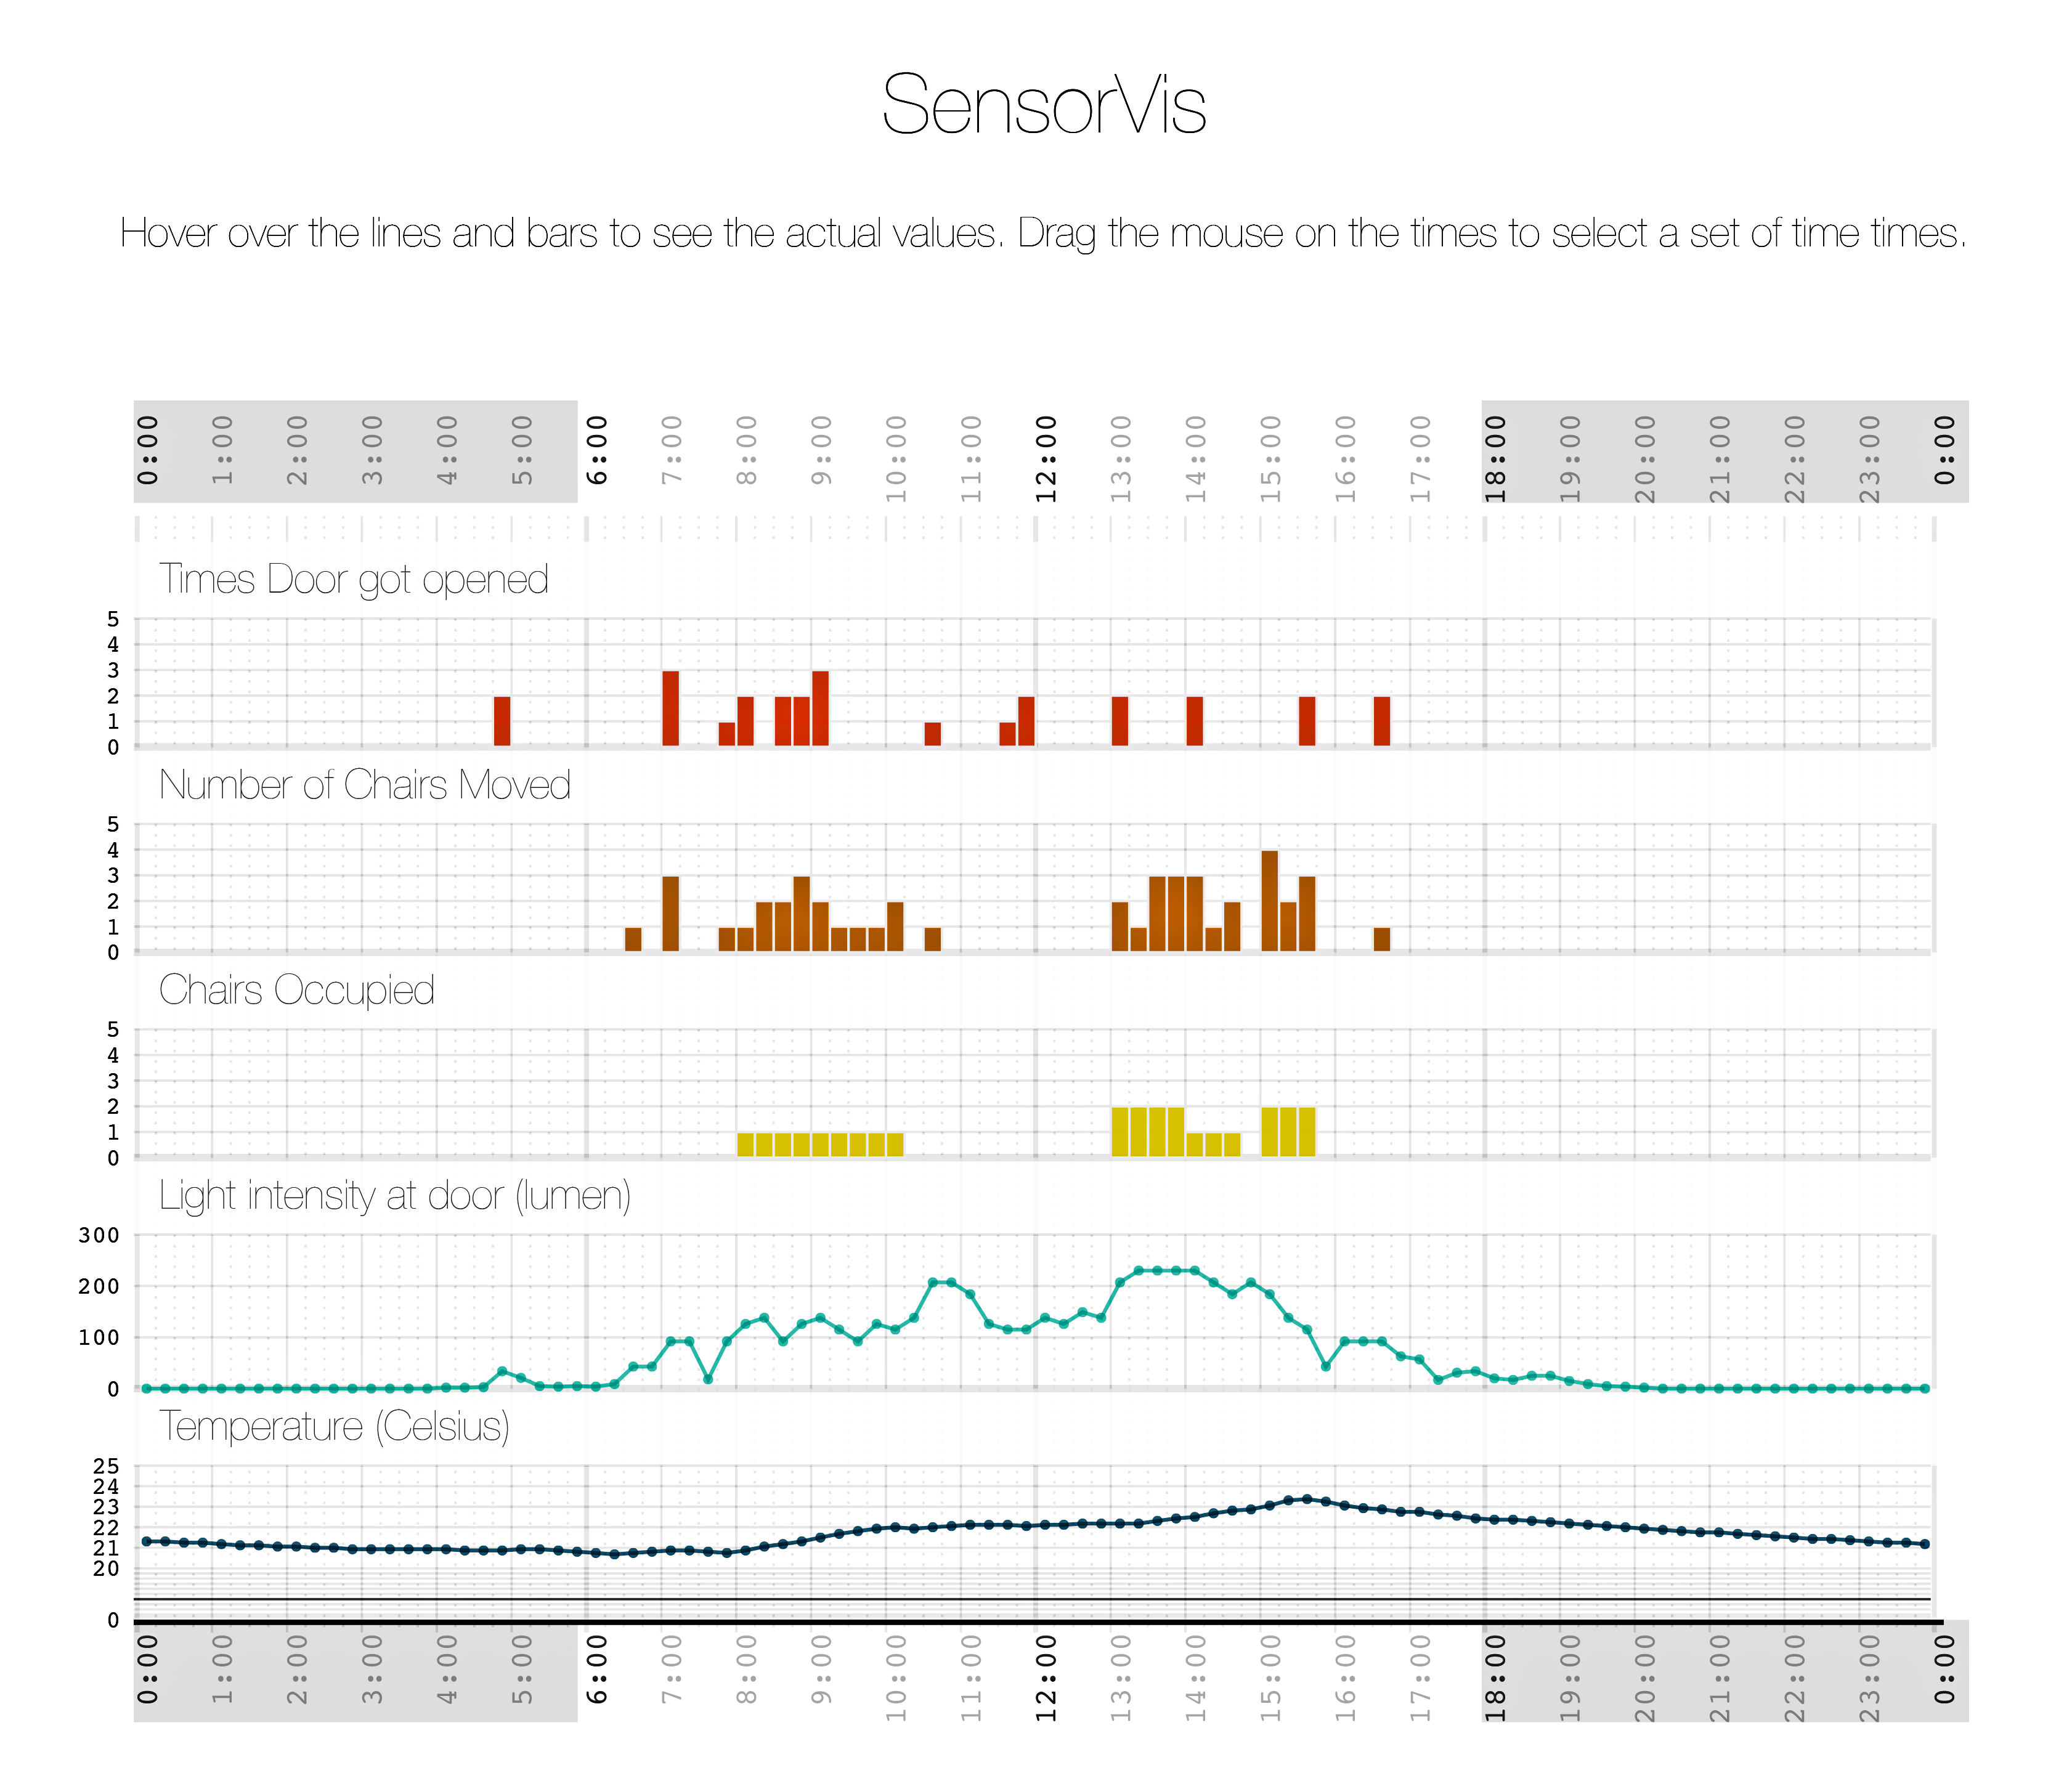
\includegraphics[scale=0.35]{images/occupancy.png}
  \caption{Screen dump of interactive data visualisation for a
    specific day. The $x$ axis shows the time dimension at 15 minute
    intervals over the course of the day. Horizontal bands show values
    for:  number of times the
    door was opened; the number of chairs that were moved; the number
    of chairs that were occupied; the light intensity in the room
    in lumens; and the temperature of the room in degrees Celsius.}
  \label{fig:dataviz}
\end{figure}
 We invited
participants to `interpret’ the data visualisation. We also asked them
whether making the monitoring data public through data visualisation
might have an impact on people’s perceptions of the monitoring and on
their ability and interest to engage with the monitoring project.

\subsection{Participant Recruitment and Data Analysis}
\label{sec:recruitment}

Our candidate pool of study participants consisted of staff based in
the offices where the monitoring project was carried out. An email
from a senior manager was sent to all staff inviting them to
participate. A separate email was sent to managers in divisions to
highlight the study and ask them to encourage their staff to engage.
Due to low initial response, additional reminders were sent out.

We recruited nine interview participants and a total of six participants for
focus groups. One of the groups consisted of two participants and the
other of four, based on staff schedules and availability. One
of the interviewees was the head of facilities management; some of the
others had heard of the monitoring project and one had seen it come
through a security review, but otherwise none of them were directly
involved with it. Four interview participants were female and five
were male. Four focus group participants were female and two were
male. We did not ask people’s ages, but a general estimate is that
most participants were between 30 and 50 years of age.

Interviews were recorded, and the transcriptions and hand-written
notes were used to analyse the data. 

%%% Local Variables: ***
%%% mode:latex ***
%%% coding: utf-8 ***
%%% TeX-engine: xetex ***
%%% TeX-master: "main.tex"  ***
%%% End: ***


\section{Results}
\label{sec:results}

\subsection{Communication}
\label{sec:communication}

One of the first questions we asked was what participants knew about
the monitoring project. Although they had all received the email that
was sent out to all staff in the building, their level of awareness of
the project depended on various factors. Some had not checked their
email and were surprised to find the sensors in the meeting rooms and
in their office space. Others knew more about it because they sat next
to people who were working on the project, were involved in some
aspect of the project themselves, or had a personal interest in the
University IoT programme and were following its activities.

\subsection{Initial Reactions to the Devices}
\label{sec:init-reactions}

A number of people were quite surprised when they discovered the
sensors%
\footnote{ 
Cf.\ the devices illustrated in figure~\ref{fig:poster}.
}
and found them rather curious, referring to them as `Pebbles’
and ‘little guys’ (Interview 2) and describing them as
`strange-coloured objects’ (Interview 2), `pink Stealth bomber’
(Interview 3), `pink lump’, `lump of flesh’ (Focus Group 2) and some
thought if they `were like little animals, like zebras or
leopards\ldots that would be more fun’ (Focus Group 2).

There were some stronger reactions to the monitoring devices that were
placed on seats, referred to as `bums on seats measurers’ (FG 2),
which people felt were fairly intrusive.

\begin{quote}I was surprised when I got down to the room that they were on the
seat part of the chair and you had to physically sit on them. That
makes me uncomfortable.\end{quote} (FG 2)

\begin{quote}It’s just too much in your personal space if it’s in
  physical contact with your rear end.\end{quote} (FG 2)

\begin{quote}It was a bit strange when you went into a meeting room…I wasn’t
expecting to sit on something, that did feel a bit weird. I’ve not
seen anything other than that that bothered me – but the sitting on
that was a bit strange. … It looks like an incontinence pad, it looks
like somebody’s going to have an accident.\end{quote} (FG 2)

\begin{quote}I didn’t like sitting on it either but I probably would have felt a
bit stupid to say I don’t really want to sit on that thing. It’s not
really any different from sitting on a chair…I don’t know, it’s…I
feel…it doesn’t know it’s [my] bum…\end{quote} (FG 2)

\begin{quote}I’ve noticed in that meeting room that I was in, people would choose
to not sit on the chair\ldots they would choose to sit on a different
chair, which I thought was quite interesting…nobody knows it’s you
sitting on the chair, it can’t read your ID card.\end{quote} (SC)

MH: snagging hose…

RG: butt sensors\ldots

Some people at first weren’t quite sure what the devices were doing.
\begin{quote}We were wondering at first what they were\ldots these strange-coloured
objects that were appearing everywhere. [We] guessed it would be
something with monitoring the room occupancy, that they would be
different types of sensors… (CM)\end{quote}

\begin{quote}\ldots it was more than you see that thing and you think, oh, is that
recording what we’re saying?\end{quote} (FG 2) 

However, with the exception of how they felt about the actual
monitoring devices, most people’s general opinion of the occupancy
monitoring project ranged from relatively neutral to enthusiastic and
supportive.

\begin{quote}I think the Internet of Things and the occupancy monitoring is fine,
because actually it’s very anonymous. It’s not being who’s in and out
or who’s part of the meeting or not – it’s just about is it being used
or is it not being used, so I think people are quite relaxed about
that kind of thing. … It was quite clearly explained and because it’s
not on desks which are allocated to fixed named individuals, there’s
no kind of data protection issues or other issues\ldots that I could see\end{quote}
(KL).

\begin{quote}I don’t think they are spying on us. It’s fairly anonymous, and what
you find out from utilisation is what it should be…\end{quote} (MF)

\begin{quote}The whole monitoring thing, I have no problem with it, because it’s
all confidential, and it’s all anonymous\end{quote} (SC)

\begin{quote}I thought it was quite exciting. I’m quite interested in technology
and how technology can be used to deliver services more easily, to
make work life easier, essentially to make things simpler. I think I
was much more on the enthusiastic positive side of it rather than
being negative.\end{quote} (GW)

\subsection{Monitoring the Meeting Room}

As conversation progressed and we got into more of the details of the
project and the issues that people experience in the building, there
were more positive reactions about the potential of the project to
deal with an identified issue. Almost everyone interviewed had
experienced some frustration with the meeting room situation in the
building.

\begin{quote}It will be quite interesting to see what’s produced at the end of it
and see what did we learn about how we use space or do we actually
occupy it when we say we’re meant to\ldots squatter people come in and use
rooms but they don’t actually book them. Often I’ll walk by and these
big rooms will be empty\ldots that’s where a lot of this can help with the
data in terms of what we do actually use it or what we don’t.\end{quote} (CM)

\begin{quote}I think it’s a great idea. I know my perception is\ldots from a
meeting-room perspective, sometimes when you look at a room like this,
there’s two people in it and you think, wait, hang on a minute, I’m
looking for a room with 25 people in it\ldots It can be quite frustrating
when you’ve got 2 people in a room of 10. Smaller rooms seem to be in
demand a lot more for 1-to-1s, half an hour slots, that kind of
thing\ldots I’ll be interested if the data you’ve been collecting shows that
the smaller rooms are actually in use as private rooms rather than the
open spaces. The [breakout spaces] are not confidential, they’re not
private enough for particular types of conversation, and the noise
carries.\end{quote} (SC)

\begin{quote}With these meeting rooms even though there will be times in the day
when some of the meeting rooms will be empty --- not all that much
because it’s very difficult to get a meeting room if you’re organising
a meeting --- it’s difficult to get a room basically for a meeting at
less than a fortnight’s notice, and I’m anticipating that will only
get more difficult as more people twig how to check all of the rooms.\end{quote}
(FG 2)

\begin{quote}I’m often booking small meetings in big meeting rooms
  down here because you do occasionally need the big rooms, but what
  we need is more rooms.\end{quote} (FG 2)

\begin{quote}I’ll book a meeting room which has got capacity of 20 just for me and
one other person because we’ve got nothing else…the occupancy is
really useful for that sort of thing because you can see, are these
large meeting rooms actually being used full all the time or are they
only getting 1 or 2 people.\end{quote} (GW)

There were multiple other building issues apart from meeting rooms
that people mentioned. Noise seemed to be a key one that was also in
part linked to the issue of meeting rooms and not having sufficient
spaces to use outside of the open plan office areas --- either for
private conversations or for louder group meetings.

\begin{quote}Are you going to do noise sensors in the offices upstairs by any
chance? When you’ve got these breakout areas, the noise rises and then
comes down, and it might help inform what you can do with the
information you’re collecting. It’s very very quiet, and that’s a
really good environment to work in, but when you get a meeting in one
of these breakout areas or one of these pods, the noise level rises
quite significantly.\end{quote} (SC)

\begin{quote}I think it would be quite good to monitor noise levels as well. This
space is a little bit tight\ldots on my floor we have a mix\ldots quite a lot of
developers and there’s also people like me that do more kind of
project management\ldots{}the developers can be quite noisy because they’re
doing a lot of this talking through stuff\ldots{}it might be better to have
everyone who needs quiet space in one area and everyone who needs
noisy space in another area. Sometimes you can have quite a lot of
interruptions, there’s just too much noise, and people are talking
about work, it’s not like they’re just messing around, it’s more like
it’s quite disturbing at times.\end{quote} (GW)

\subsection{`User' input}
\label{sec:user-input}


As mentioned in section~\ref{sec:pilot}, we used a simple data
visualisation to show people what data was being collected. The
visualisation allowed people to understand better exactly what data
was being collected and to offer their own ‘interpretation’ of it. It
also opened up opportunities for them to suggest other ways that the
data could be used to address pertinent building issues.

One thing that multiple people noticed and questioned was the data
collected on chair movement. Collecting data on chairs occupied seemed
to make sense in the context of occupancy monitoring, but it wasn’t
clear what data on chair movement would contribute to the
question. However, at least three people mentioned that the
configuration of rooms was an important issue to consider.

\begin{quote}If you could actually see how the chairs are being moved so you see
whether they get put into a theatre style so many times or whether
they get moved into circles\ldots{}I don’t know whether just knowing that
they’ve moved is that valuable, without seeing how they’ve been moved
or where they’ve been moved to.\end{quote} (GW)

\begin{quote}Actually if you had the number of chairs moved in a high level of
detail, you’d probably be able to see if someone had gone in and
reorganized the room before everybody else arrives, which would show
if they’re reconfiguring the space\ldots timetabling worr[ies] about how
much time people spend configuring space\ldots{}how effective the meeting can
be or how effective they teaching can be if you’re having to get
everybody get all the chairs and then get them in a circle and put
them all back before you can leave\ldots{}\end{quote} (CM)

\begin{quote}I come in here and do a [relaxation] class in this room\ldots{}you’re
talking about use of space, everything gets shoved to the back of the
room\ldots \end{quote} (SC)

One thought that data from the door opening and closing could provide
some interesting insights and motivation to people to arrive on time
for meetings.

\begin{quote}Ah right ok, so that’s people coming in. Interesting that they don’t
all arrive at the same time. Quite often in the University we are
terrible for starting meetings on time\ldots people drip feed their way in
after a meeting\ldots you’ll start a meeting and then someone will pop in
5, 10, 15 minutes into a meeting which can be quite disruptive,
especially if they’ve missed some key questions or key points.\end{quote} (CM)

Asking for people’s input and engaging them with the data being
collected in the project opened up a wider conversation around other
ways that data could be used. It seemed to draw out the people who had
experience in using data to design services and improve user
experience, business analytics and intelligence and environmental
monitoring, among other things. 

\begin{quote}I’m quite interested in generally understanding how students use the
University overall\ldots and why they use particular spaces within the
library over other spaces\ldots I’m also interested in\ldots how do you have an
equitable experience digitally as well as physically and what does
that mean in terms of what you need to provide for students? \ldots  I
suspect there’s some information that will be easier to get through
the Internet of things and other ways of monitoring and getting
that\ldots that will help me understand what students are doing and what
services they need. \ldots  I’m always interested in results and what we can
do to make things better.
\end{quote}
(KL) 

\begin{quote}\ldots to be able to look up some kind of app, to go, that desk is free,
that would be ideal for a lot of people who hot desk. I know upstairs
there are a lot of contractors who come in, and they’re always looking
for somewhere to sit. If the desk was free, and it could be worked in
such a way to inform some central location that the desk was
available\ldots or for two weeks because I’m going on holiday\ldots that would be
something that I think a lot of people would appreciate and benefit
from.
\end{quote}
(SC) 

\begin{quote}I would find that quite useful if you could look at the trends of
what sicknesses are in different areas or if there was any kind of
correlation between temperature and density of staff against absence
levels\ldots if you were tracking me and where I’ve been posted and my
absence record according to the different places that I’ve been
posted, you would see that in Student Systems I was off a lot, so that
would indicate there was something possibly wrong with the room or the
job. It’s that thing that we’re always trying to look for evidence and
we don’t always have quantifiable data that we can use.
\end{quote}
(CM) 

Some people didn’t find any ideas immediately coming to mind, but they
thought it would be valuable to crowd-source ideas.

\begin{quote}You could go to a community and ask for ideas\ldots explain what IoT is
about and what its current capabilities are and ask people if they’ve
got any great ideas and people start to engage at that point. Part of
it is about engaging people, trying to get people involved in the
technology as well, to raise curiosity about it. I’m sure there’s lots
of people with bright ideas who could contribute, come up with ideas.
\end{quote}
(MF) 

There was also a sense that technology initiatives could be more open.

\begin{quote}At the moment it feels like it’s all the techies --- not which it has
to be the case, because it’s new technology, and that’s the way it
always starts, but you know, the University is full of bright people,
I’m sure they could come up with a lot of bright ideas about how the
Internet of Things could be used to improve staff or student
experiences. I’m sure I’ve got two or three ideas myself\ldots I’m not sure what
they were\ldots we were talking about IoT one day and I scribbled a few
things down\ldots I think there’s definitely scope to open up in that way to
get people interested --– is to, have you got an idea for an Internet of
Things\ldots ? That would be quite fun actually.
\end{quote}
(MF) 

\subsection{``People don’t want to be reduced to numbers”}
\label{sec:people-dont-want}


While people were for the most part comfortable with the initial
monitoring project at AH, they had plenty of concerns about expanding
monitoring in the workplace, particularly if it touched on them
personally.

\begin{quote}I think there’s more issues if it were my own desk which had a
monitor attached to it. If people\ldots [are] monitoring how much I’m at my
desk, and doing X Y and Z\ldots that’s where you get into a lot of
interesting discussions about how it’s going to be used, what it’s
trying to establish – if it were trying to establish whether me and
another colleague could share a desk\ldots that might be fine, and I’m quite
up for that, but it would be about the communication back to me as an
individual\ldots whether it’s monitoring me, specifically, at that
particular point in time, that I might feel quite different about it.
\ldots Where [monitoring] is getting more difficult is if it’s
identifiable to them and their behavior, people feel less
comfortable.
\end{quote}
(KL)

\begin{quote}I suppose it’s that balance where people maybe worry about what the
consequences are – if you start monitoring someone’s usage of their
own desk, and they’re only at it 50/60\% of the time – would we opt
for hot desking, because actually we can cram 150 staff into space for
100 because nobody’s actually ever at their desk all the time. \ldots  [or]
if you’re monitoring me, are you going to tell someone that actually I
don’t turn up to my desk until 10 o’clock every day, but then maybe
work till 6\ldots how much extra information would you need to make it
valuable other than just saying the occupancy in general is X without
having any contributing factors to contextualize it, and I think
that’s where it becomes\ldots people would be a bit concerned about how it
looks, how it reflects on them, because people always think these
things are going to be negative, rather than we can learn something
from it.
\end{quote}
(CM) 

\begin{quote}I can see that I would be slightly nervous about it [if my desk was
being monitored] in the beginning, I was like, hang on, I’m being
watched, my boss could use that against me potentially\ldots I know managers
that would do that, I wouldn’t do that against my team, but then again
if I did have concerns, I might refer to it, and I think people would
be nervous of that, well hang on a minute, why weren’t you at your
desk, you’ve not got a meeting in your diary, that kind of thing.
\end{quote}
(SC)

\begin{quote}Seems to be three dimensions to it. One is, if you try to make it
less general and more specific and identify the fact that the person’s
based at a certain place, or the sex of an individual, or the age of
an individual – once you start going down that road, that’s one
dimension. The next is --– will one thing lead to another? So once you
give assent for this, will you suddenly find yourself being monitored
--– even anonymously --– for other reasons and more reasons beyond that? \ldots 
So they say they’re going to monitor the way you use your PC for one
reason – to improve efficiency –-- and then a year down the line, if
they come back and say, well, we will use this data to work out
that\ldots there’s a lot of time you’re not working, or you’re not working
on the right stuff, or you’re on your personal email too much --- all
that stuff, that side of things\ldots And also there’s no time bound --– it
seems to be, once it’s in place, it’s in place for good –-- and no one
ever seems to say it comes to an end at some point\ldots is the data going
to be kept forever, and all that stuff, and can you use that data for
other purposes than what they said?
\end{quote}
(MF)

One participant responded to the first questions about the monitoring, 

\begin{quote}I must confess, it doesn’t bother me at all. We’re getting monitored
every day, everything that we do – I’m quite used to that.\end{quote} 

But later,
when she was asked how she would feel about having her desk monitored,
she became a bit more sceptical. 

\begin{quote}Okay, so that might be slightly
different actually. I would question that I supposed. I probably would
want to understand why. As long as I was told what it was for and that
I was able to genuinely see the data that it was getting from that,
then I probably would be alright. I might say definitely if it
happens.\end{quote} (KW)

\subsection{Making monitoring acceptable}
\label{sec:making-monit-accept}

While participants expressed their concerns, they also frequently
expressed the particular reasons why they were concerned and directly
or indirectly suggested things to be done that could assuage their
concerns. They wanted to know the reason for the monitoring and how
the data was being used.

\begin{quote}[if my personal desk was being monitored] \ldots I think I’d want to know
that it was happening, and I’d want to know why it was happening, and
I would want to know how the data is being used and what use it’s
going to be put to afterwards, and what the rationale behind it was.\end{quote}
(KL)

\begin{quote}\ldots it’s when you talk about improvements --- at the moment it’s all
about collecting data --- but you’re not always sure what the purpose
is.\end{quote} (MF)

\begin{quote}I think with a lot of these things it’s just being confident that you
know what you’re signing up to, that you know what’s going to happen
to your data, and you know that if it’s going to be used in any other
way, that you’re always asked permission\ldots it’s made totally clear to
you so that you understand exactly how your data’s going to be used. I
think you have to be sort of transparent with this sort of stuff, and
I think there probably is quite a lack of trust.\end{quote} (GW)

\begin{quote}I suppose it really depends on the purpose\ldots why\ldots what would be the
purpose in collecting that information\ldots is it to see which desks are
used and which ones could be changed to hot desks and things. I
think\ldots I’d be very happy switching to a hot desk situation if there was
more flexibility about working from home\ldots I’d be very interested in a
more flexible working pattern where you could work in different
locations and not necessarily have a fixed desk.\end{quote} (GW)

They wanted the monitoring actions and the resultant decision-making
processes to be communicated clearly, and they wanted to give people
the option to participate in decision-making.

\begin{quote}The key is always being very open and transparent and really
communicating as best you can.\end{quote} (KL)

\begin{quote}You want to be efficient but you also want to be transparent, because
all you’re going to produce is data which people can use and
statistics. And statistics can be interpreted differently – there
always needs to be a context behind statistics.\end{quote} (MF) 

\begin{quote}If people know when a decision is likely to be made and to see the
outcome of participation, however small it might have been – then
people will stay interested. If it’s some nebulous affair where a
decision will be made ‘at some point’ – people won’t believe in it.\end{quote}
(MF)

\begin{quote}If they were looking into making particular decisions or changing
certain things, it would be nice to say, we’re doing x to this meeting
room, or y to this meeting room, do you agree or not agree. If there
were a number of different options for a particular meeting room, you
could see the information, see which the different options were, and
vote, have input. For me one of the more important things is to say,
we’re putting up all this monitoring stuff\ldots yes, it’s actually going
into decision making based on what we’ve found out. Otherwise why are
we bothering to do this and spend lots of time on this if we then
don’t change things and don’t act on the information?\end{quote} (KL)

They wanted to help others understand what monitoring is doing and
what it achieves.

\begin{quote}[referring to technology-enhanced learning] \ldots We’re not really
trying to profile an individual, what we’re trying to do is see what
impact this building has on people or has on a group of people, and I
think when you explain that to people then it’s usually not too bad.\end{quote}
(CM) 

\begin{quote}\ldots it’s getting away from that perception of it being a judgment –
because that’s quite often what people will think, that when you put
numbers against something they see it as being a judgment and actually
numbers are just trying to show what happens and a reflection of the
activity that goes on, and you can get insight from that that isn’t
necessarily about it being good or bad – it’s just what actually goes
on.\end{quote} (CM)

\begin{quote}I do think actually just informing people of the information that’s
being gathered and the options to help improve things\ldots I think a lot
of the time you just have to show people the benefit, rather than just
say oh, we’re collecting this. A lot of people don’t understand why.\end{quote}
(SC)



% \subsection{Management}
% \label{sec:management}

% Most people felt concerned about a variety of building issues and
% mentioned quite a few problems other than access to meeting rooms. In
% their daily experience, problems with the toilets, slow lifts, and the
% temperature of office space and of meeting rooms were significant
% complaints. In addition, the way the open plan offices were structured
% seemed to create many issues, primarily related to noise. People did
% not have private spaces to make phone calls or have one-on-one
% conversations, and informal meeting spaces in the open plan areas led
% to meetings being overheard by everyone, whether they needed to
% participate or not, and they found this disruptive to their
% work. There were also gender-related issues, such as men not wanting
% to be seen leaving early when they had the school run, or menopausal
% women needing to be able to have more control over the temperature in
% their space.  

% In terms of how building issues are managed, there were also a variety
% of complaints. Because the University is renting part of the building
% from a third party, they have less control over the management of
% building issues. Participants mentioned that the way that the
% maintenance staff treats issues can be prone to a box-ticking
% approach; for example if someone complains about the temperature in a
% space, after a few days someone will come, will measure the
% temperature at the point where air is coming out of a vent, and then
% say that everything is fine and as it should be, without considering
% the temperature in the different parts of the room where different
% people are working, or how the sun or lack thereof affects the
% temperature over the course of the day.

% People also mentioned that although there was supposed to be a
% committee of staff providing input for the design of the new
% Information Services space in Argyle House, the committee was not
% given the opportunity to provide significant input before the
% move. They were assured that after the move they would be consulted
% again, but up to the present time that had not hapened.

% Finally, some participants noted that a DIY approach to environmentla
% monitoring has already been carried out, where a few building
% occupants had designed and deployed
% their own devices (based on Raspberry Pi) to measure room temperature and
% other aspects of the working environment. 

% \subsection{Perceptions of monitoring}
% \label{sec:perc-monit}

% There were mixed perceptions of the monitoring project, and we
% identified three archetypal responses, summarised as follows: 

% \begin{enumerate}
% \item \textit{I don't care} --- I'm already being monitored in so many ways
%   that are so much more personal e.g., CCTV in the building, mobile
%   phone apps, etc. 
% \item \textit{Data is great} --- There are so many ways that we could use
%   data like this to improve our work experience. I'd
%   be happy to be monitored in even more personal ways if that would
%   bring benefit to me. 
% \item \textit{Show me the change} --- Is all this monitoring really necessary?
%   Can I see what data you’re collecting? Will the data actually be
%   used to inform a change? How will I know if it is? Might there be
%   easier or simpler ways to achieve the necessary change? 
% \end{enumerate}

% The first archetype was typically either an under- or over-informed
% person who was not likely to react negatively to the monitoring. The
% second archetype was typically a person with previous experience with
% using sensors or data analytics in their work. They were not likely to
% react negatively to the monitoring and were eager and willing to
% contribute ideas and suggestions about more monitoring options and how
% they could be used to improve user experience. The third response was
% the most common and represents people with the most potential to view
% IoT initiatives skeptically or negatively. 
% \todo{
%   Can we get incude a rough percentage of people in each of the three categories?
% }

% The majority of participants who fell in this category were
% nevertheless willing to engage or be engaged.  Management
% relationships and trust For a number of respondents, the key issues
% was the relationship between management and employees and what was
% communicated through that relationship. There was a lot of concern
% that monitoring that started out for one purpose could be exploited
% for another, depending on the type of manager.  It all depends on how
% the data is used – single biggest concern = management (not bothered
% by general environmental monitoring, but individual monitoring e.g. of
% desk use more concerning – not as much concerned about facilities
% managers as bosses) 

%%% Local Variables: ***
%%% mode:latex ***
%%% TeX-master: "main.tex"  ***
%%% End: ***

\section{Discussion}
\label{sec:discussion}

The responses of our study participants
suggest that are number of challenges to be addressed in
the successful deployment of IoT applications in offices and other
places of work.

\subsection{Privacy and Informatic Spaces}
\label{sec:privacy}

Although privacy was not a primary concern of our work with
participants, research in this area does provide some useful framing
concepts.

\cite{Jiang-2002-MPCI} introduce the notion of \term{information
    space} as ``a way to organize information, resources, and services
  around important privacy-relevant context factors.\ldots\  A
  \term{boundary}---physical, social, or activity-based---delimits an
  information space.''

In the monitoring experiment, physical boundaries were clearly
important in determining information-spaces. We chose to monitor a meeting room
specifically because it was a common space, not linked to any specific
individuals, and therefore less likely to trigger privacy
concerns. Conversely, the desks that people occupied in the open plan
offices defined a much more personal information spaces, albeit not
demarcated by such clearcut physical boundaries. 

The chairs in the monitored meeting room were somewhat less easy to
classify in this scheme. Again, they can be regarded as information
spaces, given that sensors were attached to them. And although they
are only transiently associated with any one individual (i.e., for the
duration of a meeting), at least some of the participants indicated
sensitivity about the physical closeness of the
sensors. \cite{Ohara-2016-TSVP} proposes to characterise a breach of privacy as
the state which arises when one of `my' boundaries are crossed, and if
I feel that 'my chair' or 'my-body-on-the-chair' is being monitored,
this might well be perceived as intrusive. 

O'Hara's \cite{Ohara-2016-TSVP}  approach involves seven levels of
privacy, of which the first level is occupied by the underlying concept of privacy---provisionally
identified in terms of crossing a boundary. The second privacy level concerns
the empirical facts of the matter. In terms of data protection, we
have taken care that no personal data is collected by the sensors. In
particular, the chair sensors are configured in such a way that they only allow binary
discrimination, namely was a 'sitting' event detected at a given
measuring time or not. O'Hara's third level is characterised in terms
of phenomenology: regardless of the empirical facts, how is the
situation perceived by the subject. In the case of, say, social media
platform, I may feel that I am having a private conversation with a
friend, unaware that in fact a lot of information is being collected
by the social network platform owner. However, if the presence of IoT monitoring
devices are explicitly signalled to a user, and indeed have a visible
form factor, then the converse perception of being surveilled is hard
to avoid.

In terms of a deploying an IoT monitoring system, we are therefore
confronted by the problem of a potential discrepancy between privacy
levels two and level three: we are not collecting personal data, but
the physical devices being used may prompt concerns from people that
the opposite is true. Ideally, we would like to be able to make
evident that the data flow from sensor to processing system carries no
personal information. This borrows from the notion of
\term{computational accountability} discussed in
\cite{Crabtree-2016-BAIT}: ``the surfacing or making visible of
computational behaviours or actions to better enable human-computer interactions.

\subsection{Social Context and Values}
\label{sec:social-context}

Most discussions of IoT systems and reference architectures \cite{Puschel-2016-WIAS} focus on
engineering concerns and relegate human
actors to the margins 



With top-down - or management or technophile-driven - experiments,
there is likely to be some disjunct between the vision of what could
or should be achieved (what is promised) and what is actually
delivered or accomplished. … “over-collection” of data 
…
We might define a ‘successful’ experiment as one that leads to
awareness, acceptability and trust. Or we could define it as an
experiment that either a) accomplishes the experimenter’s goals
without adverse reactions or b) involves participants in co-creating
the goals and leads to a positive experience that IoT has
‘accomplished’ something for the participants.  

We propose three principles for awareness, acceptability and trust.

\paragraph{Purpose} Monitoring should be a time-bounded activity with
a clearly defined purpose. Individuals who might be affected by the
monitoring should be informed about the what, why and how of decisions
made based on the data collected. Overmonitoring by “well-meaning
technophiles” should be avoided when simpler interventions could
achieve the desired goal. 

\paragraph{Transparency} Anyone affected by the monitoring should be
informed about what data is being collected and should be able to
access an easily interpretable explanation of this, for example
through data visualisation. Physical signage in monitored areas is
more effective than email communication. If possible, some version of
the raw data should be accessible to anyone interested in exploring it
and comparing their interpretations to that of the decision-makers. 

\paragraph{Participation} In the case of workplace monitoring, there
is an opportunity and a need to move beyond the narratives of resource
efficiency, maximising productivity and incentivising specific
behaviours. Trust in management decision-making has been compromised
by the use of data to justify cost-cutting and provide only a minimum
acceptable level of facilities and resources. 

New narratives built around trust and valuing individuals can be
created by involving employees in identifying the issues that most
affect their performance, comfort, health and well-being and
determining how and whether monitoring could be used to address these
issues effectively. The engagement process can be structured to offer
employees freedom, creativity, and a sense of agency. 

The narrative of the value of the Internet of Things to maximise
resource efficiency and improve user experience is widely embedded and
offers a seemingly easy ‘quick win’ application. However, how such an
application is designed and delivered can influence its acceptability
and either limit or expand its potential to create shared value. These
three guidelines can help to overcome skepticism and ensure that IoT
monitoring projects incorporate a broader set of values and
beneficiaries. 

%%% Local Variables: ***
%%% mode:latex ***
%%% TeX-master: "main.tex"  ***
%%% End: ***




\section{Conclusion}

\label{sec:conclusion}

Reflection on design

The original experiment was designed as a technological experiment looking for a useful application. The University was developing an IoT network and needed to look for an opportunity to test and explore the capabilities of the network in a way that would be meaningful and valuable to people. Considering the parameters of the situation, it was a well-informed choice to experiment with an identified problem that was affecting a significant group of people in their workplace, and to do this in a place (Information Services) where people would generally tend not to have adverse reactions and to be interested in the project.

The original purpose of the perceptions survey was to explore how people perceived this project and what we could learn from the project to improve design of future projects.

The principles that we identified will be valuable for future projects…

But in the process we found a deeper line of questioning and a greater opportunity to explore… We still recommend purpose / transparency / participation as guidelines for IoT projects. But we also challenge people to think from the start of an experiment not only, “how can I make this acceptable to users” or “how can I involve users” but also “what possibilities that I hadn’t imagined might arise in the process of this experiment, and how can I be alert to those, open up pathways and opportunities for unimagined possibilities to arise, and both a) empower people to innovate and b) discover new innovations in the process of a ‘standard’ experiment?



\section*{Acknowledgment}


The authors would like to thank...


\printbibliography 

\end{document}

